\documentclass[tikz,border=8pt]{standalone}
\usetikzlibrary{arrows.meta,calc}

\begin{document}
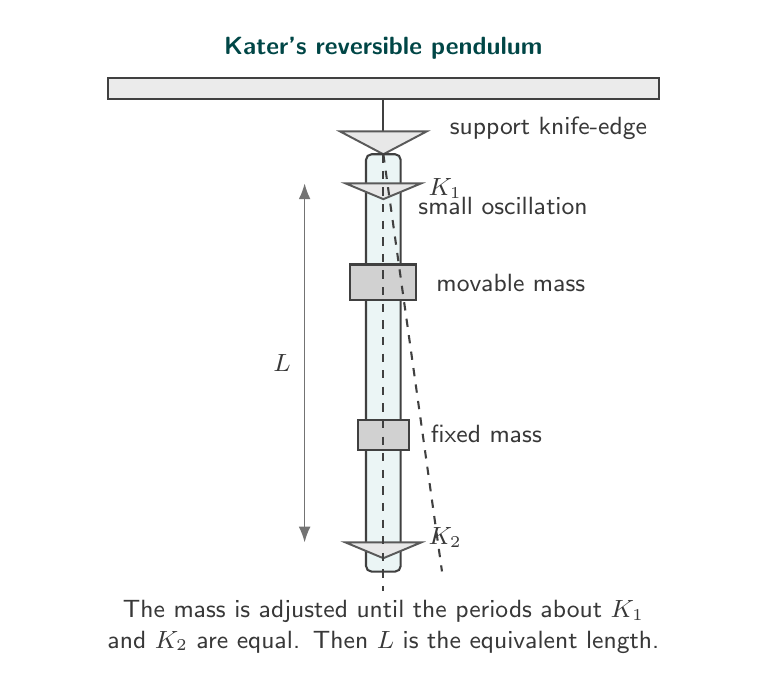
\begin{tikzpicture}[
  line/.style={draw=black!75,line width=0.75pt},
  label/.style={font=\sffamily\small,text=black!78},
  title/.style={font=\sffamily\bfseries\small,text=teal!55!black},
  knife/.style={draw=black!65,fill=black!9,line width=0.7pt},
  dim/.style={{Latex[length=2mm]}-{Latex[length=2mm]},draw=black!55,line width=0.55pt},
]

\node[title] at (0,4.0) {Kater's reversible pendulum};
\draw[line,fill=black!8] (-3.5,3.35) rectangle (3.5,3.62);
\draw[line] (0,3.35) -- (0,2.94);
\draw[knife] (-0.55,2.94) -- (0.55,2.94) -- (0,2.65) -- cycle;
\node[label,right] at (0.72,2.98) {support knife-edge};

\draw[line,fill=teal!8,rounded corners=2pt] (-0.22,2.65) rectangle (0.22,-2.65);
\draw[knife] (-0.48,2.28) -- (0.48,2.28) -- (0,2.08) -- cycle;
\draw[knife,rotate around={180:(0,-2.28)}] (-0.48,-2.28) -- (0.48,-2.28) -- (0,-2.08) -- cycle;
\node[label,right] at (0.45,2.22) {$K_1$};
\node[label,right] at (0.45,-2.22) {$K_2$};

\draw[line,fill=black!18] (-0.42,0.8) rectangle (0.42,1.25);
\draw[line,fill=black!18] (-0.32,-1.1) rectangle (0.32,-0.72);
\node[label,right] at (0.55,1.02) {movable mass};
\node[label,right] at (0.48,-0.9) {fixed mass};

\draw[dim] (-1.0,2.28) -- (-1.0,-2.28);
\node[label,left] at (-1.05,0) {$L$};
\draw[line,dashed] (0,2.65) -- (0,-2.9);
\draw[line,dashed,rotate around={8:(0,2.65)}] (0,2.65) -- (0,-2.7);
\node[label] at (1.52,2.0) {small oscillation};

\node[label,align=center,text width=8.8cm] at (0,-3.35)
  {The mass is adjusted until the periods about $K_1$ and $K_2$ are equal. Then $L$ is the equivalent length.};

\end{tikzpicture}
\end{document}
